

\section{Wizualizacja}
\label{sec:wizualizacja}

\subsection{Canvas}
\label{sec:canvas}

\subsection{SVG}
\label{sec:svg}

\subsection{SVG}
\label{subsec:svg}

Wstępny etap pracy zakładał wykorzystanie formatu SVG(en. Scalable Vector Graphics) do prezentacji danych, tworzenia animacji płynnych zmian kształtów.

Ciekawy przykład został zaprezentowany na stronie \underline{\texttt{http://www.svg-maps.com/sample\_zipcode\_map}} na której mapa po prawej stronie została w całości wygenerowana i dodano możliwość interakcji. Widok tej strony zaprezentowano na rysunku \ref{fig:svgmap}

\begin{figure}[H]
  \centering
    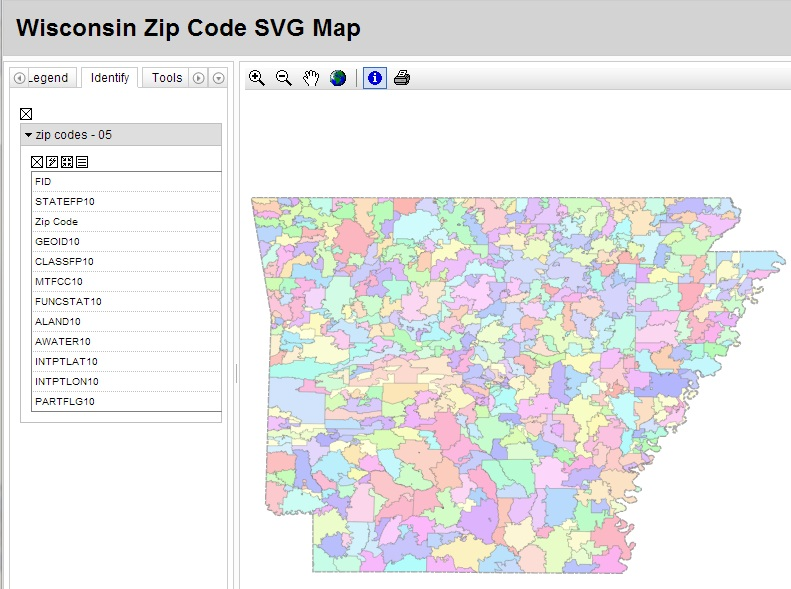
\includegraphics[width=120mm]{ge/svgmap.jpg}
  \caption{Wykorzystanie SVG}
  \label{fig:svgmap}
\end{figure}

\subsection{Canvas2}
\label{sec:canvas2}